%!TEX root = main.tex
\section{Triangulations}
\seclabel{triangulations}

%We will sometimes make use of this simple fact:
%\begin{obs}\obslabel{quad}
%	If $q=abcd$ is a simple quadrilateral, then neither of the segments $ac$
%	or $bd$ cross any of the edges of $q$.
%\end{obs}

%As is the case with \thmref{a-graph} there is an annoying case distinction
%that occurs when $Y$ contains vertices on the outer face.  

So far, we have shown that every collinear set in an A-graph is free,
and we can even specify  for edges that cross the line $Y$ the place
where this crossing occurs.
We will now apply this to prove for arbitrary planar graphs $G$
that every collinear set is free.
We might as well assume that $G$ is a maximal planar graph, i.e., a
triangulation.

% Recall that a {\em triangulation} is a (not necessarily straight-line)
% plane drawing of an edge-maximal planar graph.
% Let $T$ be a triangulation, let $r_1,\ldots,r_k$ be a sequence of vertices and edges in $T$, and let $y_1<\cdots<y_k$ be a sequence of numbers. A triangle $\Delta=\alpha\beta\gamma$ is \emph{compatible} with $r_1,\ldots,r_k$ and $y_1,\ldots,y_k$ if the following conditions hold:
% \begin{compactenum}
% 	\item if $r_1$ is a vertex, then $\beta=(0,y_1)$, otherwise $(0, y_1)$ is in the interior of the edge $r_1=\beta\gamma$; and
% 	\item if $r_m$ is a vertex, then $\alpha=(0,y_m)$, otherwise $(0,y_m)$ is in the interior
% 	of the edge $r_m=\alpha\gamma$.
% \end{compactenum}

%A triangulation is \emph{admissible} if the intersection of $Y$ with each edge of the triangulation is either empty, a single point,
%or the entire edge.

% REMINDER:
% A
% Jordan curve $C$ is \emph{admissible} for an
% embedded graph $G$ if $C(0)=C(1)$ is in the outer face
% of $G$ and the intersection between $C$ and each edge $e$ of $G$ is
% either empty, a single point, or the entire edge $e$.  


\begin{thm}\thmlabel{main}

	\begin{compactenum}
        \item Let $T$ be a triangulation,
          i.e.,
          %Recall that a {\em triangulation} is
          a (not necessarily straight-line)
plane drawing of an edge-maximal planar graph.
		\item Let $C$ be a good proper curve for $T$.
(This means that $C(0)=C(1)$ is in the outer face and the intersection between $C$ and each edge $e$ of $T$ is
either empty, a single point, or the entire edge $e$.)                  
\item Let $r_1,\ldots,r_k$ be the mixed sequence of vertices and open edges
  of $T$ that are intersected by~$C$, in the order in
  which they are intersected by $C$. Edges of $T$ that
  lie entirely on $C$
are omitted from this sequence.
(They are implicitly represented by their endvertices, which are two consecutive elements $r_i$ and $r_{i+1}$.)
		\item Let $y_1<\cdots<y_k$ be a sequence of numbers.
%		\item let $\Delta$ be a triangle that is compatible with %
%    $r_1,\ldots,r_k$ and $y_1,\ldots,y_k$.
                  
                \item Let $\epsilon>0$ be a tolerance parameter.
\end{compactenum}
Then
%        , for any $0<\epsilon<\min\{(y_{i+1}-y_i)/3:i\in\{1,\ldots,k-1\}\}$,
        $T$
        has a \Fary\ drawing such that,
        %the outer face is delimited by $\Delta$ and such that the
        %following hold
        for each $i=1,\ldots,k$: 
	\begin{compactenum}[a)]
		\item if $r_i$ is a vertex, then it is drawn at $(0,y_i)$; and
		\item if $r_i$ is an edge, then the intersection of $r_i$ with $Y$ has $y$-coordinate in the interval $[y_i-\epsilon,y_i+\epsilon]$.
\end{compactenum}

Moreover, we can specify the shape $\Delta$ of the outer triangle,
subject to
obvious compatibility constraint that it intersects $Y$ in the specified points.
                
\end{thm}
The last condition can be formulated more precisely:
We say that the triangle $\Delta=\alpha\beta\gamma$ is \emph{compatible} with the
given data $r_1,\ldots,r_k$ and $y_1,\ldots,y_k$ if the following conditions hold:
\begin{compactenum}
	\item if $r_1$ is a vertex, then $\beta=(0,y_1)$, otherwise $(0, y_1)$ is in the interior of the edge $r_1=\beta\gamma$; and
	\item if $r_m$ is a vertex, then $\alpha=(0,y_m)$, otherwise $(0,y_m)$ is in the interior
	of the edge $r_m=\alpha\gamma$.
\end{compactenum}

If the tolerance $\epsilon$ is large, 
the statement of the theorem allows the order in which the edges cross
$Y$ to change. This is not intended, and it can be excluded it we choose
$\epsilon<\min\{(y_{i+1}-y_i)/2:i\in\{1,\ldots,k-1\}\}$. In the proof,
we will actually make this assumption.

\begin{proof}
	%   We call $y_i$ the (desired) \emph{crossing coordinate} for $r_i$. If
	%   a \Fary\ drawing contains an edge whose intersection with the
	%   $y$-axis is $\{(0,y)\}$ or a vertex at $(0,y)$, we say that the edge
	%   or vertex \emph{crosses the $y$-axis at $y$}.
	%
	%   Let $L=C^-$, $R=C^+$.  
  We start by classifying the edges of $T$.  An edge that has one
  endpoint in $C^-$ and the other endpoint in $C^+$ is a \emph{crossing
    edge}, otherwise it is a \emph{non-crossing edge}.

  An edge
  is \emph{marked} if it intersects $C$, otherwise it is
  \emph{unmarked}.  The unmarked edges are completely disjoint
  from~$C$.  The marked edges include all crossing edges, but also the
  edges with one endpoint on $C$ and the edges that lie completely on
  $C$.
	
	%   We prove an extension of the theorem to the case where $T$ is an
	%   non-crossing embedded graph whose faces consist of triangles (3-cycles)
	%   and quadrilateral (4-cycles) with the resriction that, for every
	%   quadrilateral face $q$, all four edges of $q$ are crossing edges.
	%   The proof is by induction on the number of non-crossing edges plus the
	%   number of vertices of $T$.
	
	%   \paragraph{Base Cases:}
	%   There are three base cases tht we handle explicitly.  If $T$ contains
	%   2 or fewer crossing edges, If $T$ is the complete graph, $K_4$ on 4
	%   vertices, but only has only three crossing edges, then the theorem is
	%   also easy to prove directly.  The last base case occurs when all edges
	%   of $T$ are crossing edges.  In this case $T$ is bipartite and therefore
	%   all its faces are quadrilaterals, so $T$ is a quadrilateralization.
	%   This case is handled directly by \lemref{quad2}.
	%
	%   Thus we may assume that $T$ has at least one non-crossing edge and
	%   at least 2 crossing edges.  
	
	The proof is a double induction on the number of vertices of $T$, primarily, and on the number of non-crossing edges of $T$, secondarily.
	We begin by describing reductions that allow us to apply the
	inductive hypothesis. When none of these reductions applies,
	we arrive at our base case. To handle the base case,
	we remove every unmarked edge of $T$ to obtain an A-graph, to which we
	apply \thmref{a-graph}.

% we argue that
%	$T$ has a sufficiently simple structure that it can be handled by
%	\thmref{a-graph}.  In particular, when no reduction applies, we can
	
%	Before continuing, we dispense with one easy special case.  If $Y$
%	contains an edge $e$ of the outer face, then every vertex
%	of $G$ is contained in $L\cup Y$ or every vertex of $G$ is contained
%	in $Y\cup R$.  In this case, the definition of compatible triangle
%	implies that the edge $\alpha\beta$ of $\Delta$ is contained in the
%	$y$-axis.  In this case, we can simply apply Tutte's Convex Drawing
%	Theorem to obtain a \Fary\ drawing of $G$ in which the outer face is embedded
%	on $\Delta$ with $e$ embedded on $\alpha\beta$, .  This drawing
%	satisifies all the conditions of the theorem.  Therefore, for the
%	remainder of this proof, we assume that $C$ intersects the interior
%	of at least one inner face of $T$.
	
\paragraph{Separating Triangles.}
(See \figref{separating}.)
	If $T$ contains a separating triangle $xyz$, then denote by
        $T^+$ (respectively, $T^-$) the triangulation obtained from
        $T$ by removing all the vertices in the interior
        (respectively, exterior) of $xyz$. The triangle that $xyz$ delimits an
        inner face of $T^+$ and the outer face of $T^-$.
Both $|V(T^+)|<|V(T)|$
and $|V(T^-)|<|V(T)|$, so we can apply induction if necessary.
        
The case that the interior of $xyz$ does not intersect $C$ is easy.
We draw $T^+$ by induction.  In this drawing, % of $T^+$,
we take the triangle representing the cycle $xyz$, and we draw $T^-$
so that its outer face coincides with this triangle, for example by
Tutte's Convex Drawing Theorem~\cite{tutte:how}.

Consider now the case that $C$ intersects the interior of $xyz$. Then
$C$ intersects the boundary in two points: either it passes through a
vertex of $xyz$ and the opposite open edge, or it intersects two open
edges of $xyz$. %, each in a single
% point, and does not intersect the third edge of $xyz$.
% with each of $xy$, $yz$ and $zx$ is either empty or a single point. 
In both cases, the vertices and edges of $T$ intersected by $C$ that
are not in $T^+$ form a nonempty contiguous subsequence
$r_i,\ldots,r_j$ of $r_1,\ldots,r_k$. Each of $r_{i-1}$ and $r_{j+1}$
is either an edge or a vertex of $xyz$.
	
	\begin{figure}
		\centering{\includegraphics{figs/separating}}
		\caption{Recursing on separating triangles in the proof of
			\thmref{main}}
		\figlabel{separating}
\end{figure}
	
%Set $\epsilon'$ to be any
%	value less than $\min\{\epsilon,y_{i}-y_{i-1},
 %       y_{j+1}-y_j\}$.
Apply induction on $T^+$ with the value $\epsilon':=\epsilon/2$ and the sequences $r_1,\ldots,r_{i-1},r_{j+1},\ldots,r_k$ and
	$y_1,\ldots,y_{i-1},y_{j+1},\ldots,y_k$. In the obtained \Fary\ drawing of $T^+$ let $\Delta'$ be the triangle representing  $xyz$ and let $y_{i-1}'$ and $y_{j+1}'$
	be the respective $y$-coordinates of the intersections of
	$r_{i-1}$ and $r_{j+1}$ with $Y$.  By the choice of
	$\epsilon'$ we have $y_{i-1}'<y_i<\cdots<y_j<y_{j+1}'$.  Observe that
	$\Delta'$ is compatible with $r_{i-1},\ldots,r_{j+1}$ and
	$y_{i-1}',y_i,\ldots,y_j,y_{j+1}'$.
	%
	We apply induction on $T^-$ with value $\epsilon$ using the triangle $\Delta'$ and the sequences $r_{i-1},\ldots,r_{j+1}$ and
	$y_{i-1}',y_i,\ldots,y_{j},y_{j+1}'$.  Combining the \Fary\ drawings of $T^+$
	and $T^-$ yields the desired \Fary\ drawing of $T$.  Thus,
        from now on we assume that $T$ has no separating triangles.
	
	\paragraph{Contractible Edges.}
	(See \figref{contractible}.)
	A face of $T$ is a \emph{crossing
		face} if it is incident to two crossing edges. We declare an
	unmarked edge of $T$ to be \emph{contractible} if it is not contained
	in the boundary of any crossing face.  
	\begin{figure}
		\centering{\includegraphics{figs/contractible}}
		\caption{Contracting and uncontracting edges in the proof of
			\thmref{main}}
		\figlabel{contractible}
	\end{figure}
	
	If $T$ contains a contractible edge $xy$ then we contract $xy$ to
	obtain a new vertex $v$ in a smaller triangulation $T'$.   We then apply
	induction on $T'$ with the value $\epsilon'=\epsilon/2$ to obtain a \Fary\
	drawing of $T'$ such that each crossing edge $e_i$ crosses
	$Y$ in the interval $[y_i-\epsilon/2,y_i+\epsilon/2]$.
	
	To obtain a \Fary\ drawing of $T$ we uncontract $v$ by placing $x$ and $y$
	within a ball of radius $\epsilon/2$ centered at $v$. (Such
	a placement is always possible, by a standard argument, see, e.g.,~\cite{fary,w-sp-05}.)  Since the
	distance between $y$ and $v$ and the distance between $x$ and $v$ are each at most $\epsilon/2$,
	each crossing edge $r_i$ incident to $x$ or $y$ crosses $Y$ in the interval $[y_i-\epsilon,y_i+\epsilon]$, as required.
	Thus, in the following we assume that $T$ has no separating triangles or contractible
	edges.
	
	%   \paragraph{Eraseable edges}
	%   We say that a non-crossing edge of $xy$ of $T$ is \emph{eraseable}
	%   if neither of its endpoints is on $C$ and both its incident faces
	%   intersect $C$.  If $T$ contains an eraseable edge $xy$, then we remove
	%   the edge $xy$ from $T$ to obtain smaller graph $T'$ on which we can
	%   apply induction. In the resulting drawing of $T'$, $x$ and $y$ lie on
	%   a common face (which may be the outer face of $T'$) and are visible.
	%   We can therefore add the edge $xy$ to obtain the desired drawing
	%   of $T$.
	
\paragraph{Flippable edges.}
	(See \figref{flippable}.)
	We declare an unmarked edge $xy$ of $T$ to be \emph{flippable} if there
	exist distinct vertices $z$, $a$, $b$, and $c$ such that:
\begin{compactenum}[(11) ]
\item [(1)]
  $xyz$ is a non-crossing face of $T$;
\item [(2)]
  $xyb$, $zyc$, $xza$ are crossing faces of $T$;
  and either 
\item [(3a)] $C$
        intersects $za$, $xa$, $xb$, $yb$, $yc$, and $zc$ in this
        order, or
      \item [(3b)] $C$ intersects $xa$, $xb$, $yb$, $yc$, $zc$,
        and $za$ in this order. (This case can only occur when
        $xza$ is the outer face, otherwise $xza$ would be a separating
        triangle.)
        \end{compactenum}

        
	\begin{figure}
		\centering{\includegraphics{figs/flippable}}
		\caption{Flipping edges in the proof of
			\thmref{main}. Top row: Case 3a. Bottom row:
                        Case~3b}
		\figlabel{flippable}
	\end{figure}
	
	If $T$ contains the flippable edge $xy$ then we remove $xy$ and replace it with $zb$ to obtain a new triangulation $T'$. Note that, since $T$ has no separating triangles, the edge $zb$ is not already present in $T$. Further, $T'$ has the same number of vertices of $T$ and one less non-crossing edge. After choosing a crossing coordinate $y_{zb}$ for $zb$ between those $y_{xb}$ and $y_{yb}$ of $xb$ and $yb$, we can inductively draw $T'$ with tolerance $\epsilon$ and sequences $r_1,\dots,xb,zb,yb,\dots,r_k$ and $y_1,\dots,y_{xb},y_{zb},y_{yb},\dots,y_k$.
	
We claim that in the resulting \Fary\ drawing of $T'$,
% the only open edge that intersects the open segment $xy$ is $zb$.
we can replace $zb$ by $xy$ without creating a crossing, thus producing
 the desired \Fary\ drawing of $T$.
%
We show this by establishing that both $b$ and $z$ are convex vertices in $xbyz$.
The vertex $b$ is not a reflex vertex in $xbyz$, since $bx$ and $by$ are crossing
edges.
                In Case~(3a), the existence of the
	edges $za$ and $zc$ ensures that, in the \Fary\ drawing of $T'$,
	$xbyz$ is convex. In Case~(3b), the triangle $zxa$ is convex
        and $xbyz$ is contained in this triangle, therefore $z$ is
        a convex  vertex in $xbyz$.
        %In either case, removing $zb$ from the \Fary\ drawing of $T'$ and replacing it with $xy$ yields the desired \Fary\ drawing of $T$.
	
	\paragraph{Edges on $C$.}
	
	If $T$ contains an edge $xy$ that lies on $C$, then we treat it as we treated flippable edges. In this case, $xy$ is incident to two triangles $xyz$ and $yxb$ with $z\in C^+$ and $b\in C^-$. We replace $xy$ with an edge $zb$ to obtain a new triangulation $T'$ with the same number of vertices of $T$ and one less non-crossing edge. We apply induction and get a \Fary\ drawing of $T'$, in which $z$ and $b$ are
	on opposite sides of $Y$ and $x$ and $y$ are on $Y$, hence 	neither $z$ nor $b$ is a reflex vertex of the quadrilateral $xzyb$.
	Thus, removing $zb$ and adding $xy$ gives a \Fary\ drawing of $T$.
	
	\paragraph{The Base Case.}
	
	We are left with the case in which $T$ is a triangulation
	with no separating triangles, no contractible edges, no flippable
	edges, and no edge contained in $C$.  If $T$ is the complete graph
	on three or four vertices, then the proof is trivial,
	so we may assume that $T$ has at least 5 vertices.

        We will simply omit the marked edges. The result will be an
        A-graph, to which we can apply \thmref{a-graph}. In the
        resulting drawing, we will see that we can reinsert the
        omitted edges without producing crossings.

        
	\begin{claimx} \label{unmarked}
	Any unmarked edge $xy$ in $C^+$ is on the boundary of two
        faces $xyz$ and $yxb$ where $z,b\in C \cup C^-$,
see \figref{two-triangles}a--b.
      \end{claimx}

      \begin{figure}[htb]
        \centering
        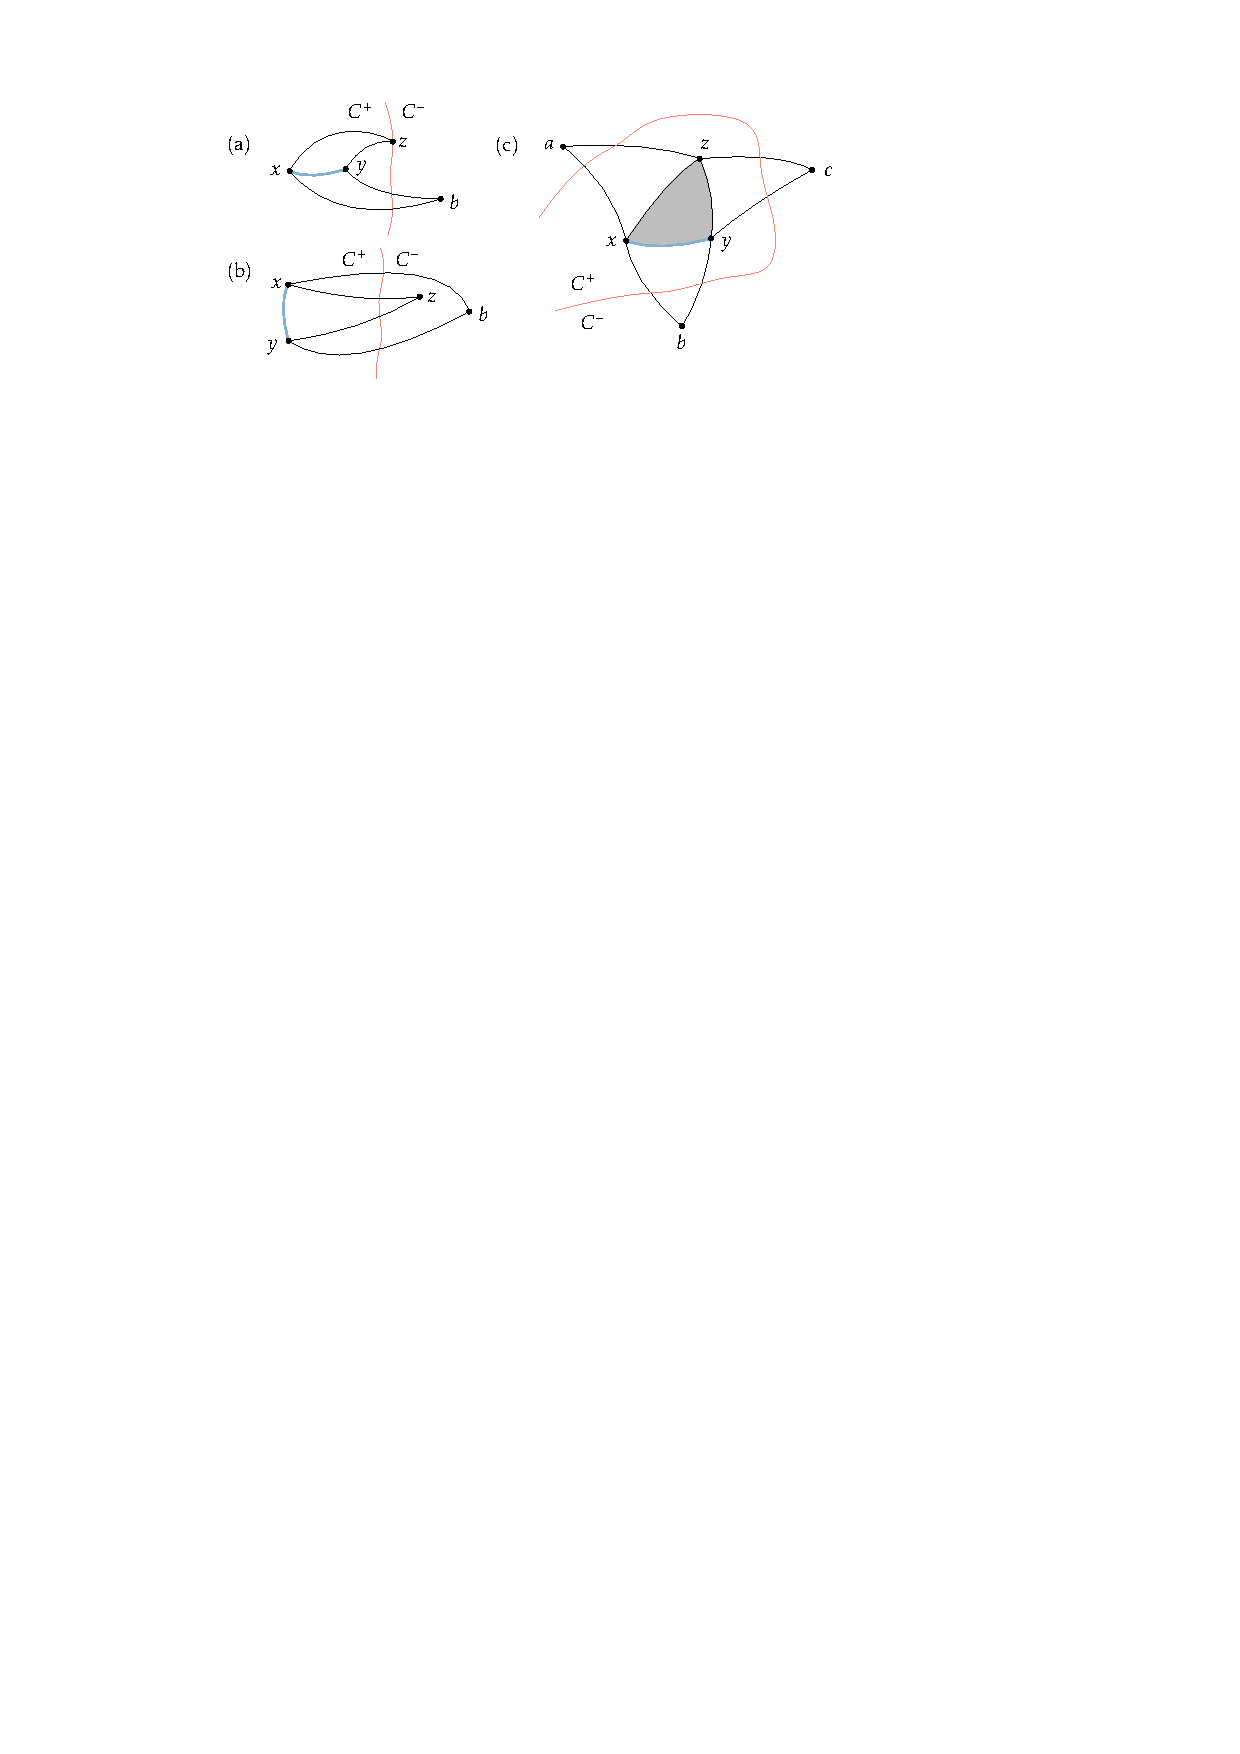
\includegraphics{figs/unmarked}
        \caption{(a--b) The two triangles incident to an unmarked edge
          $xy$.
          In case (b), $yxb$ is the outer face.
          (c) The triangles adjacent to $xyz$ in the proof of Claim
\ref{unmarked}.
        }
        \label{fig:two-triangles}
      \end{figure}
		
	\begin{proof}
	Since $xy$ is not contractible, at least one of $xyz$ and $yxb$ is a
	crossing triangle, so at least one of $z$ and $b$, say $b$, is in $C^-$.
	Suppose then, for the sake of contradiction, that $z\in C^+$. Since neither $zx$ nor $yz$ is contractible,
	they must be incident to crossing faces $xza$ and $zyc$, respectively,
see \figref{two-triangles}c.
	If $a=b=c$, then $T$ is the complete graph on four vertices,
	which we have already ruled out.  Therefore, assume without loss of
	generality that $b\neq c$.  %Since $T$ contains no separating triangles,
	We have $a\neq c$, because otherwise $xya$ would
be a separating triangle that
        separates $z$ from $b$. Similarly, $a\neq b$, otherwise $byz$ would separate $x$ from $a$.	
	This leaves us in the situation in which we have distinct vertices $x$,
	$y$, $z$, $a$, $b$, and $c$ such that $xyz\in C^+$, such that $xyb$, $zyc$, and $xza$
	are crossing faces of $T$, and such that $xyz$ is a non-crossing face of $T$.
	Then at least one of $xy$, $yz$, or $zx$ is a flippable edge. This contradiction proves the claim.
\end{proof}	

	Symmetrically, every unmarked edge $xy$ in $C^-$ is incident to two faces
	$xyz$ and $yxb$ with $z,b\in C \cup C^+$.  This implies that no face of $T$ contains more than one unmarked edge.
	
	Thus, every unmarked edge of $T$ is incident to two faces that intersect $C$. The union of these two faces is a quadrilateral whose boundary consists of four edges that intersect $C$.
	Let $\tilde{G}$ denote the plane drawing obtained by removing all unmarked edges
	from $T$.  By \thmref{dujmovic-frati}, we know that $\tilde G$ has
	a \Fary\ drawing $G$ whose edges and vertices intersect $Y$ in the
	same order as they intersect $C$ in $\tilde{G}$. We have the following.
	
	\begin{claimx} \label{claim-a-graph}
		$G$ is an A-graph.
	\end{claimx}
	
	\begin{proof}
In order to	prove the claim, we check each of the properties of an A-graph
	(\defref{a-graph}).
	\begin{compactenum}
		\item The removal of unmarked edges and the fact that $T$ has no
		edge entirely on $C$ ensures that every edge of $G$ intersects $Y$
		in exactly one point.
		\item Because no face of $T$ is incident to more than one unmarked edge,
		each face of $G$ is a quadrilateral or a triangle.  
		\item A quadrilateral face $q=abcd$ appears in $G$ when we remove the unmarked edge $ac$ from $T$. This, and the fact that every edge of $q$ intersects $Y$, ensures that $a$ or $c$ is a reflex vertex of $q$.
		\item The only triangular faces of $G$ are those consisting
		of three marked edges, which necessarily have one vertex in
		each of $Y$, $L$, and $R$.
		\item Since $T$ has no edge on $C$, every vertex of $T$ on $C$
		is incident to two triangular faces (one above and one below)
		each having three marked edges. These faces are still present in $G$.
	\end{compactenum}
This concludes the proof of the claim.
\end{proof}	

	%
	%The graph $Q^*$ has two triangular faces $vab$
	%   and $vcd$ incident to $v$ such that $ab=r_{i-1}$ and $cd=r_{i+1}$.
	%   Split $v$ into two vertices $x\in L$ and $y\in R$ joined by the edge
	%   $xy$, make $x$ adjacent to all neighbours of $v$ in $R$, and make
	%   $y$ adjacent to all neighbours of $v$ in $L$. See \figref{split}.
	%   This splitting operation eliminates the triangular faces $vab$ and
	%   $vcd$ and introduces the quadrangular faces $xyab$ and $yxcd$.
	%
	%   \begin{figure}
	%      \centering{
	%        \begin{tabular}{c|c}
	%            \includegraphics{figs/split} & \includegraphics{figs/split-outer}
	%        \end{tabular}}
	%      \caption{Splitting vertices on $C$ in the proof of
	%      \thmref{main}.}
	%      \figlabel{split}
%   \end{figure}

We would now like to apply \thmref{a-graph} to obtain a \Fary\ drawing
of $G$ in which, for each $i\in\{1,\ldots,k\}$, the intersection of
$r_i$ with $Y$ is at $(0,y_i)$ and the appropriate vertices on the
outer face of $T$ map to the vertices of the triangle $\Delta$.
Before doing so, we must first prescribe an outer face $\Delta'$ for
the \Fary\ drawing of $G$.  If the outer face of $G$ is a 3-cycle,
then we use $\Delta'=\Delta$.  Otherwise, suppose the outer face of
$G$ is a 4-cycle $\alpha x\beta\gamma$ and $\alpha\beta$ is an
unmarked edge of $T$.  In this case, the locations of $\alpha$,
$\beta$, and $\gamma$ are given by the three vertices of $\Delta$
(with $\alpha$ and $\beta$ both on the same side of $Y$).
If $x$ lies on $Y$,
then $x=r_i$ for some~$i$, %\in\{1,\ldots,k\}$ or the position of $a$ is
and the
position of $x$ is determined by $y_i$.
Otherwise, it is determined
by the positions of $\alpha$ and $\beta$ and the values
$y_{i}$ and $y_j$ where $r_i=\alpha x$ and $r_j=\beta x$.

	In this way, we can apply \thmref{a-graph} to
	obtain a \Fary\ drawing of $G$ in which the intersection of $r_i$
	with $Y$ is at $(0,y_i)$.  Each internal edge $ac$ of $T$ not in $G$
	corresponds to a quadrangular face $q=abcd$ of $G$ in which $a$ or $c$ is a
	reflex vertex.  Therefore, the edge $ac$ can be added to the drawing
	without introducing crossings.  A single external edge $\alpha\beta$
	on the outer face of $T$ might not appear in $G$. In this case the outer
	face of $G$ is a quadrilateral $q'=\alpha x \beta \gamma$ in which $x$ is
	a reflex vertex, so the segment $\alpha\beta$ lies outside of $q'$, and the edge $\alpha\beta$ can therefore be added to the drawing of $G$
	without introducing crossings. Therefore reinserting each edge of $T$ not in $G$ gives the desired \Fary\ drawing of $T$ (and the choice of $\Delta'$ ensures that the outer face of this drawing is $\Delta$). 
        This concludes the proof of \thmref{main}.
\end{proof}
	
We are finally ready to prove \thmref{our-bang}. Given a plane drawing
of a graph $G$, a collinear set $S$ in $G$,
	and any $y_1'<\cdots<y_{|S|}'$, we need to prove that $G$ has
	a \Fary\ drawing in which the vertices in $S$ are drawn at
	$(0,y_1'),\ldots,(0,y_{|S|}')$. If $G$ is not a
        triangulation. Indeed, we add edges to it
so that it becomes a triangulation.
By \thmref{collinear-set},
the property that $S$ is collinear set is  preserved.
%After
% constructing a \Fary\ drawing in which the vertices of $S$ are
% positioned at $(0,y_1'),\ldots,(0,y_{|S|}')$, the inserted edges can
% be removed, and we obtain the desired \Fary\ drawing of the initial
% graph.
 % Assume hence that $G$ is a triangulation.
 \thmref{dujmovic-frati} implies
	that there exists a Jordan curve $C$ that is admissible for $G$
	and that contains all the vertices of $S$ in some order, say
	$v_1,\ldots,v_{|S|}$.  The curve $C$ intersects a subset of the edges
	and vertices of $G$ in some order $r_1,\ldots,r_k$.  We choose any
	sequence $y_1<\cdots<y_k$ so that, for all $i\in\{1,\ldots,k\}$ and
	$j\in\{1,\ldots,|S|\}$, $y_i = y_j'$ if $r_i=v_j$.  We select
	any triangle $\Delta$ that is compatible with $r_1,\ldots,r_k$ and
	$y_1,\ldots,y_k$ and choose $\epsilon = (1/3)\min\{\,y_{i+1}-y_{i}:
	i\in\{1,\ldots,k-1\}\,\}$.  \thmref{main} then gives us a \Fary\
	drawing of $G$ in which the vertices in $S$ are at
        $(0,y_1'),\ldots,(0,y_{|S|}')$, as required by
        \thmref{our-bang}.
Finally, edges that were inserted to create a triangulation are simply removed, and we obtain the desired \Fary\ drawing of the initial graph.



%%% Local Variables:
%%% mode: latex
%%% TeX-master: "freecoll"
%%% End:
